\section{Paradoja de EPR}

% Partamos, suponiendo que la mecánica cuántica es una teoría local, de modo que 

Si tenemos dos partículas entrelazadas, sabemos que al medir una de ellas, se definirá en un estado, y por tanto, la otra también lo hará. El problema con esto, es que, aparentemente, tenemos dos eventos directamente relacionados, ocurriendo al mismo tiempo, lo que parece una contradicción a la Relatividad.

% Veamos cual es el error de este planteamiento; para que la mecánica cuántica siga las reglas de la Relatividad, debe ser una teoría local, y por tanto

% \input{Geogebra/EPR-Bell.tex}

\begin{figure}[H]
    \centering
    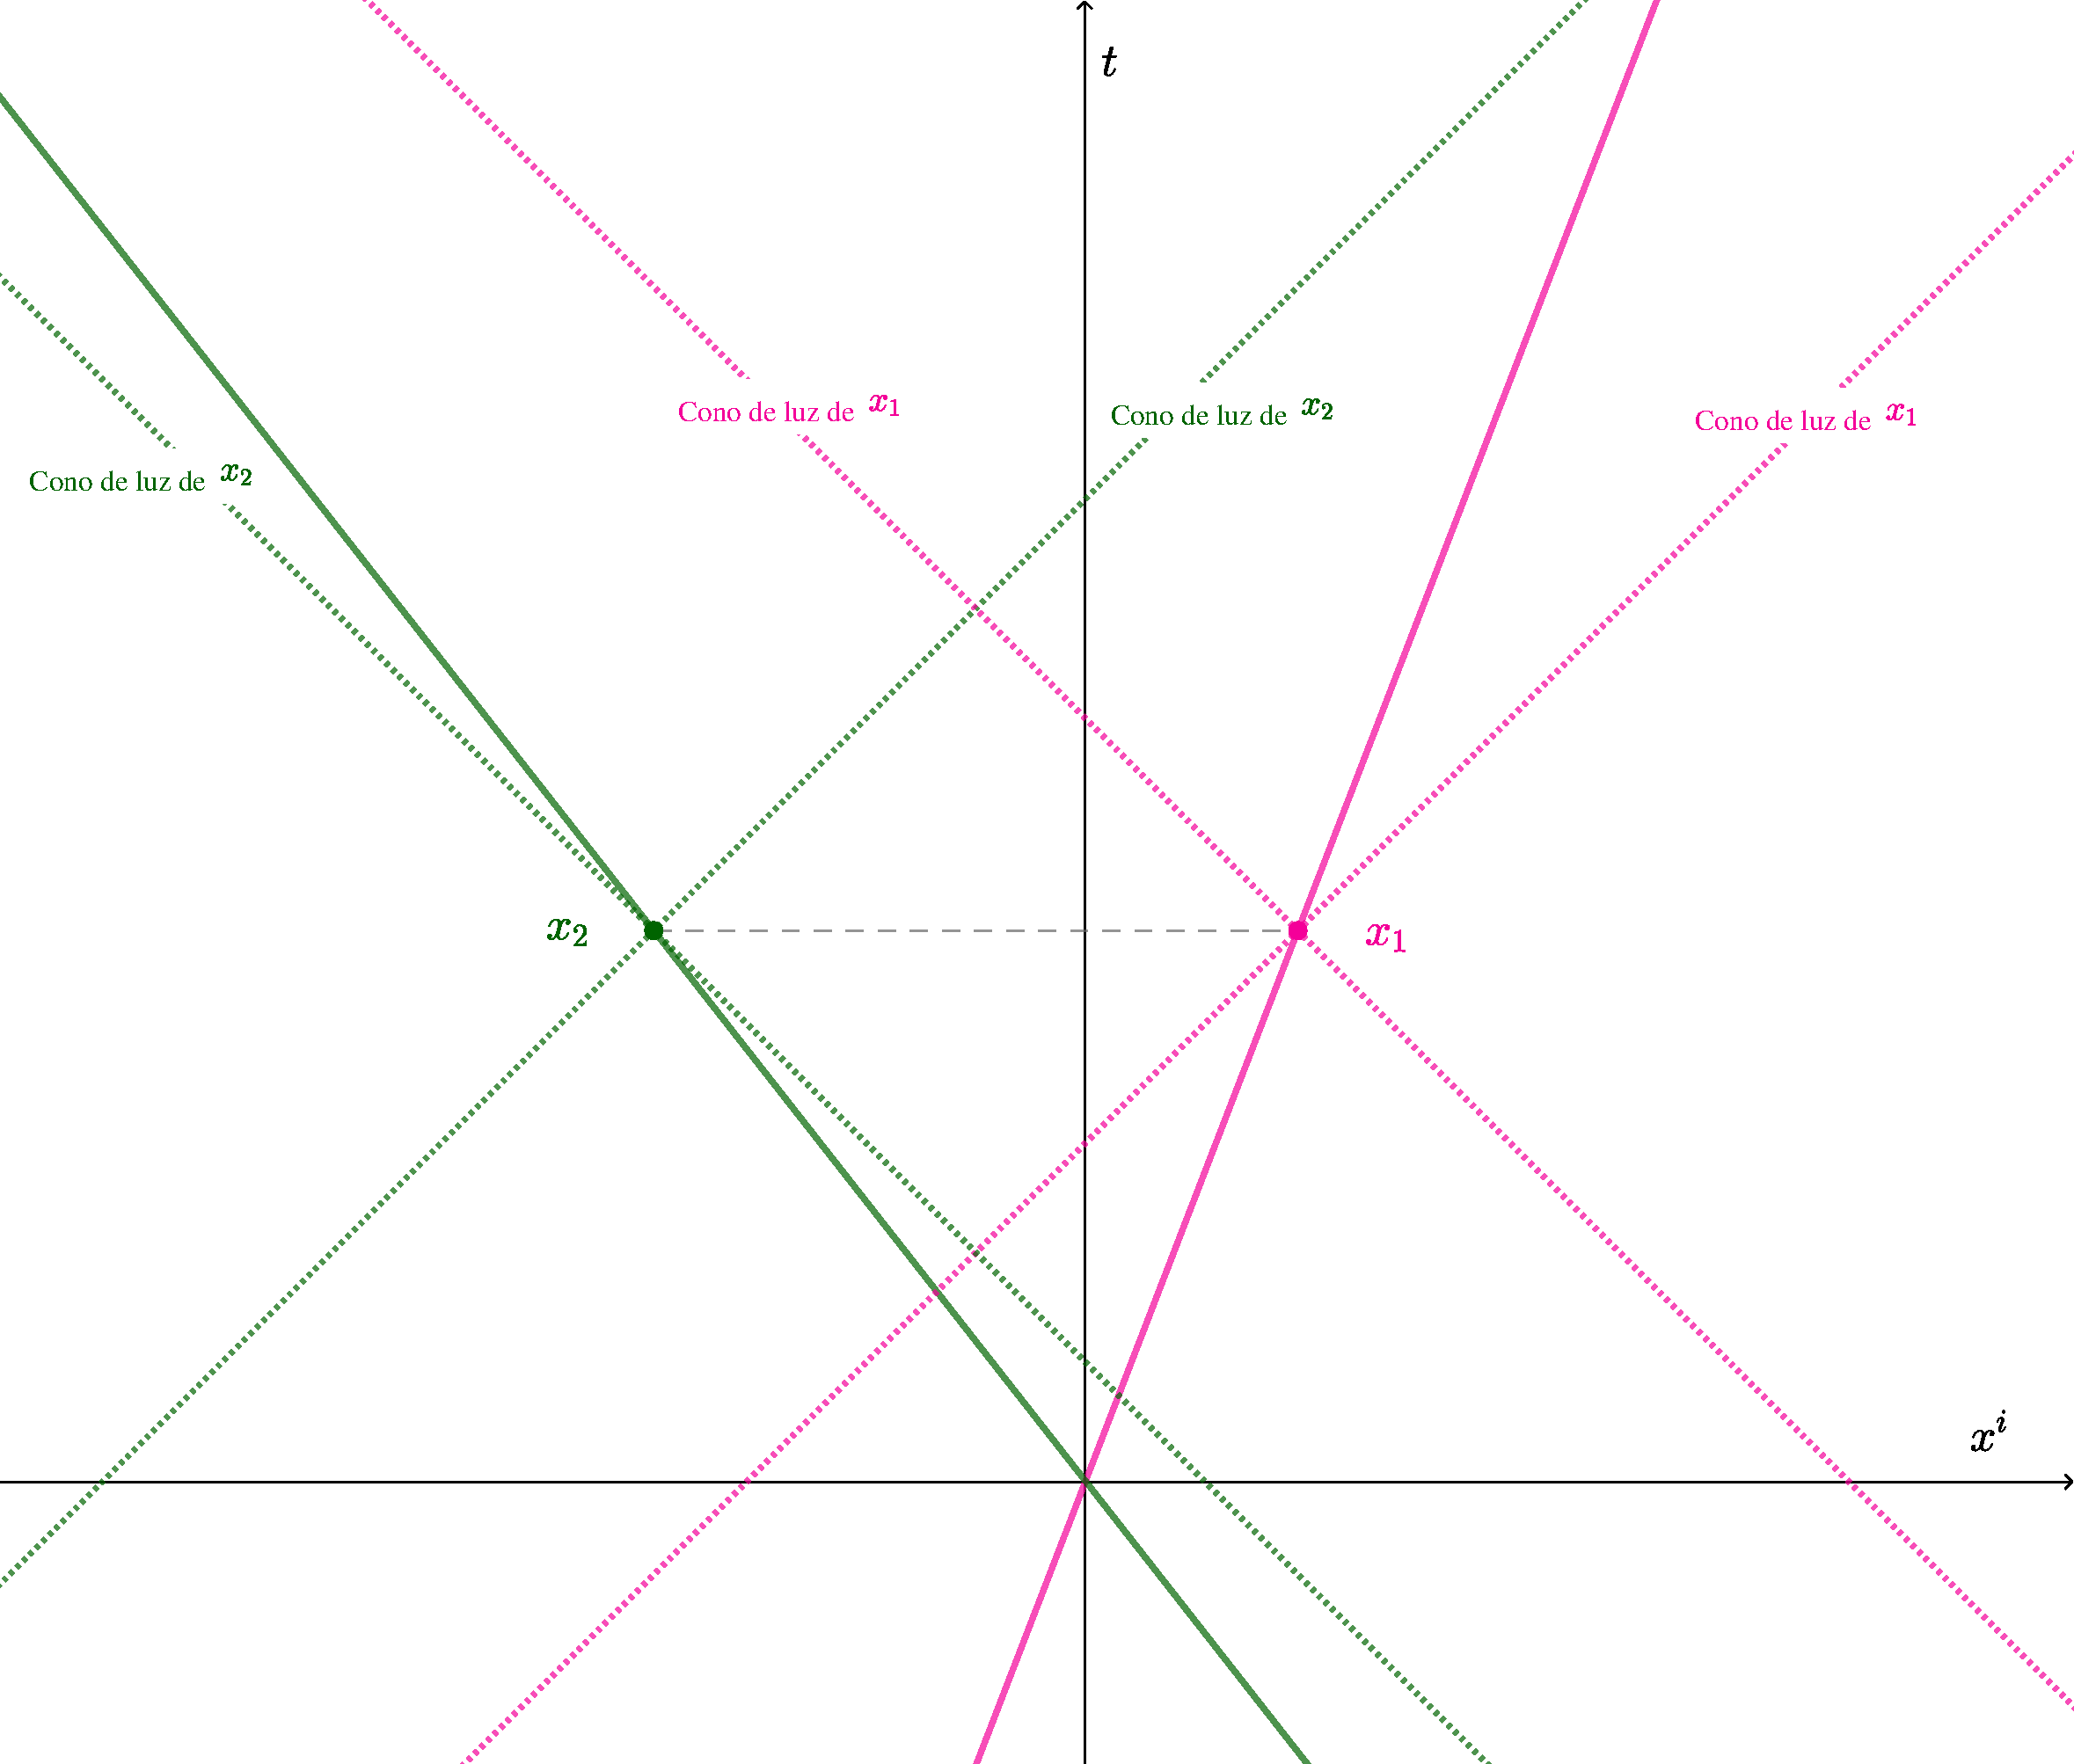
\includegraphics[width=0.8\textwidth]{Graphics/SpaceLike.pdf}
    \label{fig:SpaceLike}
    \caption{Diagrama de Minkowski}
\end{figure}
\bigskip

Veamos este planteamiento con más rigurosidad matemática:

\medskip

Sean $\mathbf{x_1}$ y $\mathbf{x_2}$, dos partículas observadas por un mismo observador en un sistema inercial, que se entrelazan en $t=0$ y luego se alejan a velocidades $\mathbf{v_1}$ y $\mathbf{v_2}$ respectivamente. Entonces tenemos:

\begin{align*}
    \mathbf{x_1} &= \left(x^0_1,x^1_1,x^2_1,x^3_1\right)\\
    \mathbf{x_2} &= \left(x^0_2,x^1_2,x^2_2,x^3_2\right)
\end{align*}

Pero, al ser observados por un mismo observador, partiendo de un mismo evento, entonces: $x^0_1=x^0_2=t$:

\begin{align*}
    \mathbf{x_1} &= \left(t,x^1_1,x^2_1,x^3_1\right)\\
    \mathbf{x_2} &= \left(t,x^1_2,x^2_2,x^3_2\right)
\end{align*}

Y suponiendo una velocidad constante, entonces $x^i_n=tv^i_n$:

\begin{align}
    \mathbf{x_1} &= \left(t,tv^1_1,tv^2_1,tv^3_1\right)\\
    \mathbf{x_2} &= \left(t,tv^1_2,tv^2_2,tv^3_2\right)
\end{align}

Calculemos entonces $\Delta x^\alpha$

\begin{align*}
    \Delta x^\alpha 
        &:= \left(x^\alpha_2-x^\alpha_1\right)\\
    \Delta x^0
        &= \left(t-t\right)=0\\
    \Delta x^i
        &= \left(x^i_2-x^i_1\right)\\
        &= \left(tv^i_2-tv^i_1\right)\\
        &= t\left(v^i_2-v^i_1\right)\\
        &= t\Delta v^i
\end{align*}

Calculemos ahora $\Delta s^2$

\begin{align*}
    \Delta s^2 
        &:= -\eta_{\alpha\beta}\Delta x^\alpha \Delta x^\beta\\
        &=-\eta_{00}~\cancelto{0}{\left(\Delta x^0\right)^2}-\cancelto{\delta_{ij}}{\eta_{ij}}~~~~~\left(\Delta x^i\Delta x^j\right)\\
        &=0-\delta_{ij}\left(\Delta x^i\Delta x^j \right)\\
        &=\sum_{i=1}^3-\left(\Delta x^i\right)^2\\
        &=-t^2\sum_{i=1}^3 \left(\Delta v^i\right)^2\\
        &=-t^2\left[\left(\Delta v^1\right)^2+\left(\Delta v^2\right)^2+\left(\Delta v^3\right)^2\right]\\
        &\leq0
\end{align*}

El caso de la igualdad solo se da en $t=0$ o si las velocidades de ambas partículas son las mismas, de modo que $\Delta v^i = 0~~\forall~i\in[1,3]$

Y por tanto, en el caso que las velocidades sean distintas, la métrica de Minkowski es menor a cero, es decir, los eventos $x_1$ y $x_2$ no tienen una relación causal. Y al estar correlacionados, esto es una aparente violación de la teoría de la Relatividad.

